\chapter{RELATED STUDY}

The aim of software security is that software continues to function correctly even while under attack. Memory errors do not always expose a way for an attacker to exploit them but even in these cases an attacker could potentially exploit these problems in order to perform a very effective denial of service attack. However, when memory errors in programs exposed to the internet are exploitable, they can lead to the attackers gaining control over an entire systems. So from a safety viewpoint it is also very important to make sure these types of errors are found and fixed. Or mitigated some other way, for example with dynamic checks around memory access. This means that not using static analysis may make software much more vulnerable to attacks, than if a static analysis tool was used that can detect various issues.

C and languages similar to it employ manual memory management. These types of languages are not memory safe languages as they require the programmer to explicitly request and free memory when needed instead of the language taking care of it automatically. C and C++ are examples of these kind of, memory unsafe languages. 

The most common issues, in not memory safe languages, are array bounds checking problems (buffer overflow and underflow), not releasing memory (memory leak), releasing memory too soon (also called dangling pointers), and problems with using uninitialized data. 

This study aims to create a static analysis tool for detecting buffer overflow vulnerabilities.

\section{STATIC ANALYSIS APPROACH}
Sophisticated techniques couple static code analysis with formal methods. Formal methods apply theoretical computer science fundamentals to solve difficult problems in software, such as proving that the software will not fail with a run-time error. The combination of static code analysis and formal methods enables developers to detect difficult to find errors and prove the absence of certain types of bugs/errors. E.g. these techniques can prove that the following line of code will never fail with a divide by zero run-time error. Most of today’s tools for static analysis function in basically the same way. They receive code as input, build a model that represents the program, perform some sort of analysis in combination with knowledge about what to search for and finally present the result to the user. Figure \ref{fig:st_analyse} shows the process that all static analysis tools that target security make use of.

\clearpage

\begin{figure}[!htbp]
    \centering
    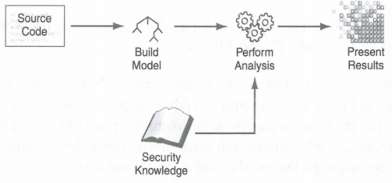
\includegraphics[width=0.8\textwidth]{Imgs/st_analyse.png}
    \caption{\label{fig:st_analyse} Generalized view of the process of a static analysis}
\end{figure}


The first step taken by the tools when performing an analysis is to build a model of the program. In this way an abstract representation of the program is created, which is better suited to be used for the actual analysis and what kind of model that is created depends largely on what kind of analysis that is to be performed. The simplest model, used in a lexical analysis, is a stream of tokens. This is created by taking the source code first. Then discarding all unimportant features such as white spaces and comments and finally translates all parts of the code into tokens.

This stream can then be used to perform a simple lexical analysis on. The next step is to translate the stream of tokens into a parse tree by using a parser that matches the token stream against a set of production rules. The parse tree contains the most direct representation of the code just as the programmer wrote it and can thus be used as a good base to perform analysis.

However, since the production rules might intro duce various symbols in order to make the parsing easy, a parse tree is not the best representation to perform more complex analyzes on. The next step is instead to translate the parse tree into an AST as well as creating a symbol table alongside it. These can then be used as input to a semantic analysis of the program. Another thing that the AST might be used for is to scan it by using predefined patterns in order to find errors that require data-flow analysis of the code. This is not possible to perform on for example a token stream. The procedure of performing a static analysis is until now very alike the procedure taken by a compiler when compiling a program.

But as a compiler as a next step will use the AST to generate an intermediate representation of the code, which can be used for optimization and later on translation to platform specific code, the processes now separates. Most of the tools instead continue by building a control flow graph, which can be used to inspect the various paths in the program or to track data flow, on top of the AST. The way the graph is used by a tool depends largely on which techniques the tool makes use of and this has a big impact on efficiency, speed and result of a scan.

Another thing that influences the result of a scan is how the tool makes certain simplifications of the program. The very essence of a static analyzer is that the program being analyzed is not run. However, in order to perform a through scan the tool, as already described, translates the code into an abstract representation and then “executes” the program on an abstract machine with a set of non-standard values replacing the standard ones. This is where a concept referred to as states is introduced. States are a collection of program variables and the association of values to those variables. 

For every program statement the state of a variable may change in some way and the aim for a static analysis is to associate the set of all possible states with all program points. 

The use of states and how a tool makes the approximations and the simplified descriptions of sets is something that makes the tools differs greatly from one and another. Some make very sophisticated and accurate decisions in order not to make unjustified assumptions about the result of an operation whilst others resort to a more simple approach. This incremental approach goes against what almost everyone in the industry tries to do, especially with security. As the code is being developed, it needs to be brought under the security policy, quality policy, whatever in every single day. If they keep on top of it, it hardly impacts the team’s workflow at all. In fact, it actually saves them time when you factor in the benefits of the error prevention it delivers. But if they allow it to lapse, catching up becomes too overwhelming. \cite{Five}

\section{EXISTING BUFFER OVERFLOW DETECTION METHODS}
\subsection{ARCHER (Array Checker)}
ARCHER is a constraint solver tool that checks the bounds of the variables and memory
sizes of various objects. ARCHER statically analyzes the source code for memory constraint violations such as array accesses, pointer dereferences, or calls to a function that expects a size parameter.

\subsection{BOON (Buffer Overrun Detection)}
BOON was developed to detect buffer overflows using integer range analysis. This is achieved by parsing through the program looking for string variables. When found, string variables are assigned two integers. The first integer is the string’s allocated size, and the second is the number of bytes currently in use. Then, the algorithm checks the usage of each string to determine if the length of the string is greater than the size allocated for the string.

\subsection{UNO (Uninitialized Variables, Nil-Pointer Dereferencing, And Out of Bound Array Indexing)}
In other buffer overflow detection techniques, false positives are common. UNO is a tool that aims to reduce the number of false positive reported and to allow users to define their own application-dependent properties for checking for flaws. As its name indicates, the tool checks for errors such as uninitialized variables, nil-pointer dereferencing, and out of bound array indexing. UNO is an extension of a tool called ctree, which produces a parse tree of a program. UNO runs the ctree program to get a parse tree, then converts the tree into a control flow graph. Once the graph is created, UNO performs its buffer overflow analysis on the control flow graph. Overall, UNO requires two passes through the code. The first pass is to build the tree and graph, and then check for errors.

\subsection{Value Set Analysis}
Value set analysis is the technique of recovering “information about the contents of machine registers and memory locations at every program point in an executable”. This technique was used by Kindermann to perform buffer overflow detection via the static analysis 7 of executables. This buffer overflow detection method focused on the detection of buffer overflows caused by loops.
\cite{Four}.